\chapter{État de l'art}

\index{état de l'art}
\index{méthode}

\section{Travaux existants}

Les capteurs QCM sont utilisés, entre autres, pour la mesure de l'épaisseur de films rigides. Les quartz peuvent également être immergés pour la détection de gaz et de liquides.

\subsection{Contrôle du dépôt par évaporation thermique}

Le dépôt par évaporation thermique est utilisé pour déposer des couches minces de matériaux sur des substrats.  
Les microbalances sont utilisées pour surveiller en temps réel la masse déposée sur le substrat, en analysant la variation de fréquence du cristal de quartz.  
Cette technique est particulièrement utile pour la fabrication de dispositifs électroniques, optiques et de capteurs.

\fig[H, width=12cm]{Dépôt par évaporation thermique \cite{inficon_selectionguide_lesker}}{Dwg-ID-FILMTHICKMONCONTROLCOMPONENTS.svg}

\subsection{Détection d'huiles}

Les microbalances à quartz peuvent être recouvertes d'un film d’un matériau sensible aux huiles,  
comme le montrent les travaux de Triyana et al. \cite{triyana2019highly}, où un capteur QCM est utilisé pour détecter la présence de safrol.  
Les capteurs ont été recouverts de nanofibres de PVAc au moyen d’un procédé d’électrofilage, ainsi que d’un film de PVAc par la méthode de \textit{spin-coating}.  
Les molécules de safrol s’attachent aux molécules de PVAc, ce qui modifie la masse adsorbée sur le cristal de quartz,  
et donc la fréquence de résonance du cristal.

\begin{figure}[H]
    \centering
    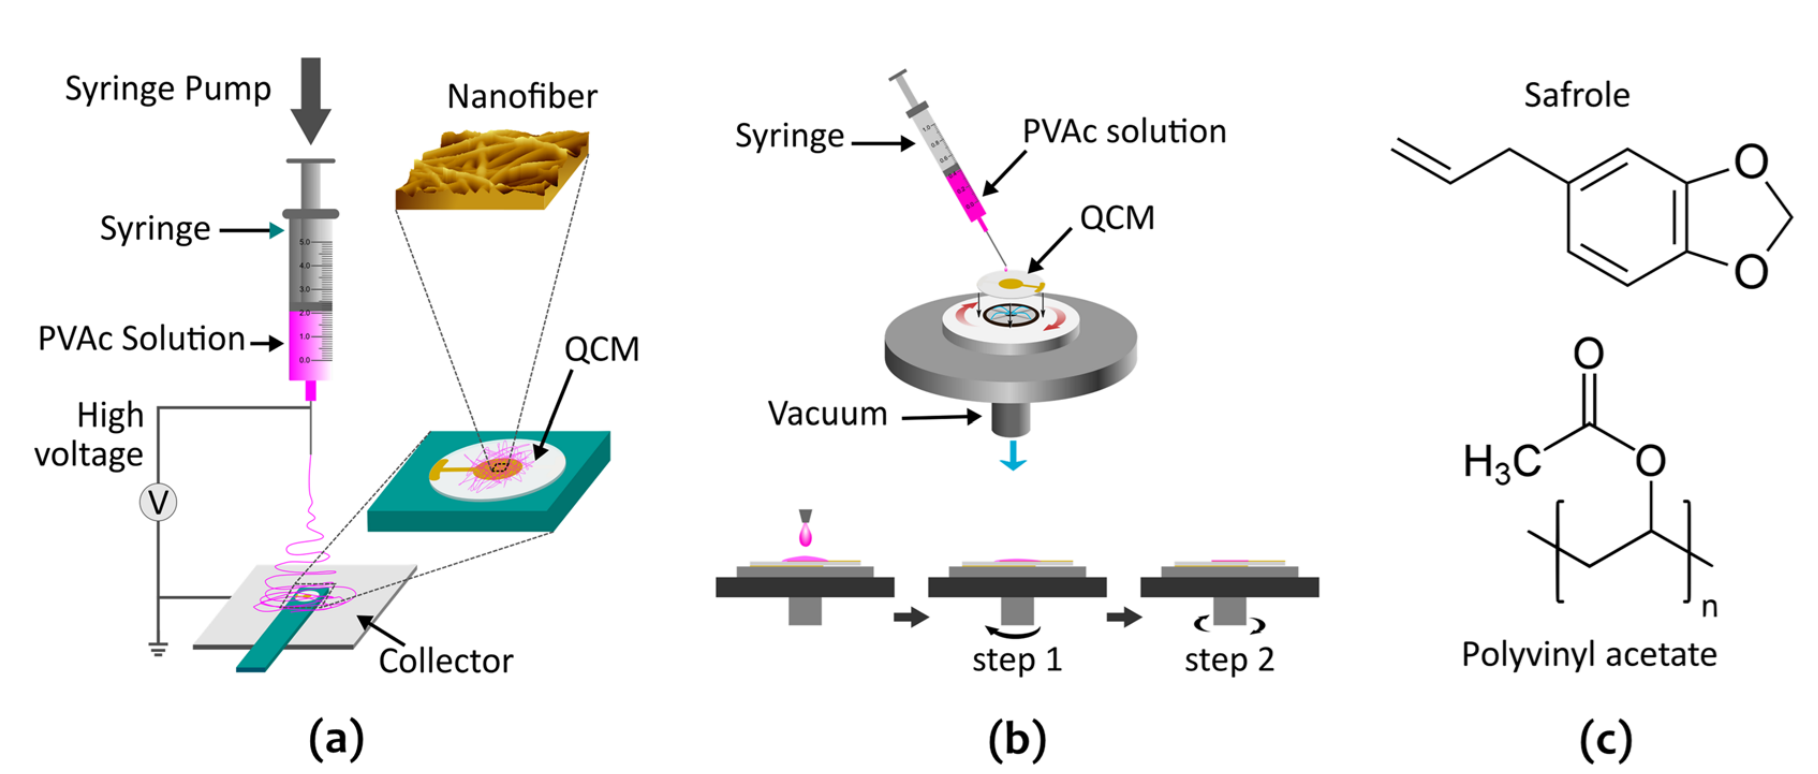
\includegraphics[width=0.8\textwidth]{assets/figures/Safrol Sensor.png}
    \caption{Détection de l'huile dans l'eau avec un capteur QCM \cite{triyana2019highly}.}
    \label{fig:Safrol_detection}
\end{figure}

\subsection{Détection de méthane}

Les microbalances peuvent aussi être utilisées pour détecter des gaz dissous dans un liquide.  
Une étude publiée dans le journal \textit{ACS Applied Nano Materials}, visant à détecter la présence de méthane dans l’eau de lac \cite{doi:10.1021/acsanm.4c06883},  
montre qu'il est possible de le faire avec une grande sensibilité.

Les capteurs QCM ont été recouverts de matériaux poreux de type MOF (Metal-Organic Framework).  
Ces matériaux offrent des propriétés permettant une réponse rapide (moins de 60 secondes) et une sensibilité à l’échelle des parties par milliard.

\begin{figure}[H]
    \centering
    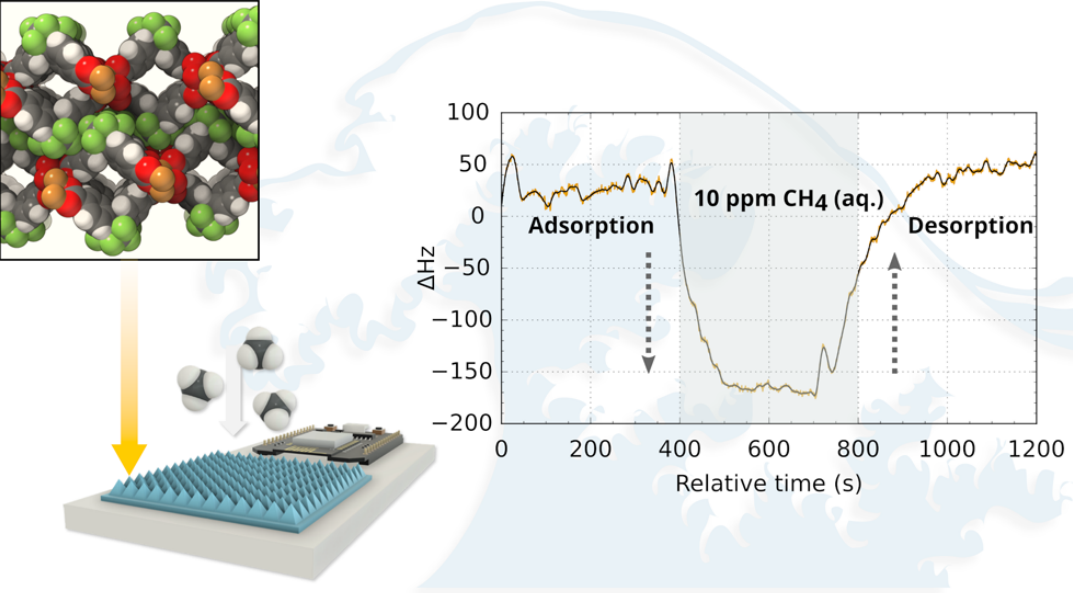
\includegraphics[width=0.8\textwidth]{assets/figures/methane sensor.png}
    \caption{Détection du méthane dans l'eau avec un capteur QCM \cite{doi:10.1021/acsanm.4c06883}.}
    \label{fig:methane_detection}
\end{figure}

\section{Technologies et méthodes existantes}

\subsection{Phénomène piézoélectrique}

Le phénomène piézoélectrique est la capacité de certains matériaux à générer une charge électrique lorsqu’ils sont soumis à une contrainte mécanique.  
Inversement, ces matériaux peuvent également se déformer lorsqu’ils sont soumis à un champ électrique.

Dans le cas des microbalances à cristal de quartz (QCM), les deux phénomènes sont utilisés.  
Le quartz est excité à une fréquence électrique qui le fait vibrer mécaniquement.  
Il émet ensuite un signal électrique qui varie selon la masse adsorbée sur sa surface et les propriétés du milieu dans lequel la mesure est effectuée.

\subsection{Coupe du quartz}

Les coupes des cristaux de quartz sont définies selon les axes cristallins principaux du quartz.  
Un nombre infini de coupes est théoriquement possible. Cependant, certains angles de coupe présentent des propriétés particulières qui les rendent plus adaptés à certaines applications.  
Les coupes les plus courantes sont les coupes AT, BT et ST.

Dans notre cas, nous utiliserons la coupe AT, qui est la plus répandue pour les applications de microbalances à cristal de quartz (QCM), en raison de sa stabilité thermique.

\begin{figure}[H]
    \centering
    \begin{minipage}[t]{0.48\textwidth}
        \centering
        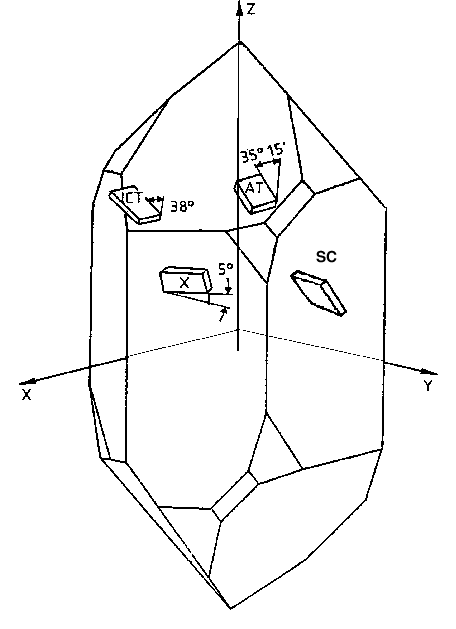
\includegraphics[width=\textwidth]{assets/figures/Orientation-of-different-cuts-in-a-natural-quartz-crystal.png}
        \caption{Différentes coupes de quartz dans un cristal naturel.}
        \label{fig:quartz_cuts}
    \end{minipage}
    \hfill
    \begin{minipage}[t]{0.48\textwidth}
        \centering
        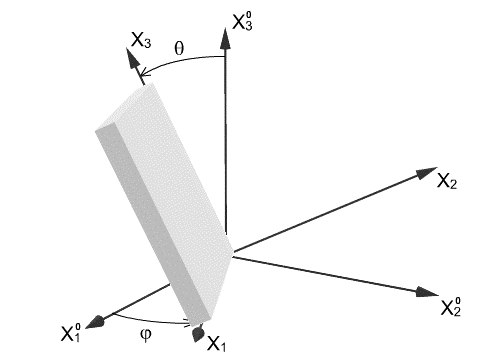
\includegraphics[width=\textwidth]{assets/figures/ph-and-th-cut-angles.png}
        \caption{Angles de coupe du quartz.}
        \label{fig:cut_angles}
    \end{minipage}
\end{figure}

\subsection{Sensibilité du capteur QCM}

Le quartz présente une sensibilité suivant une distribution gaussienne de la masse adsorbée sur la surface du cristal \cite{s22145112}.

\begin{figure}[H]
    \centering
    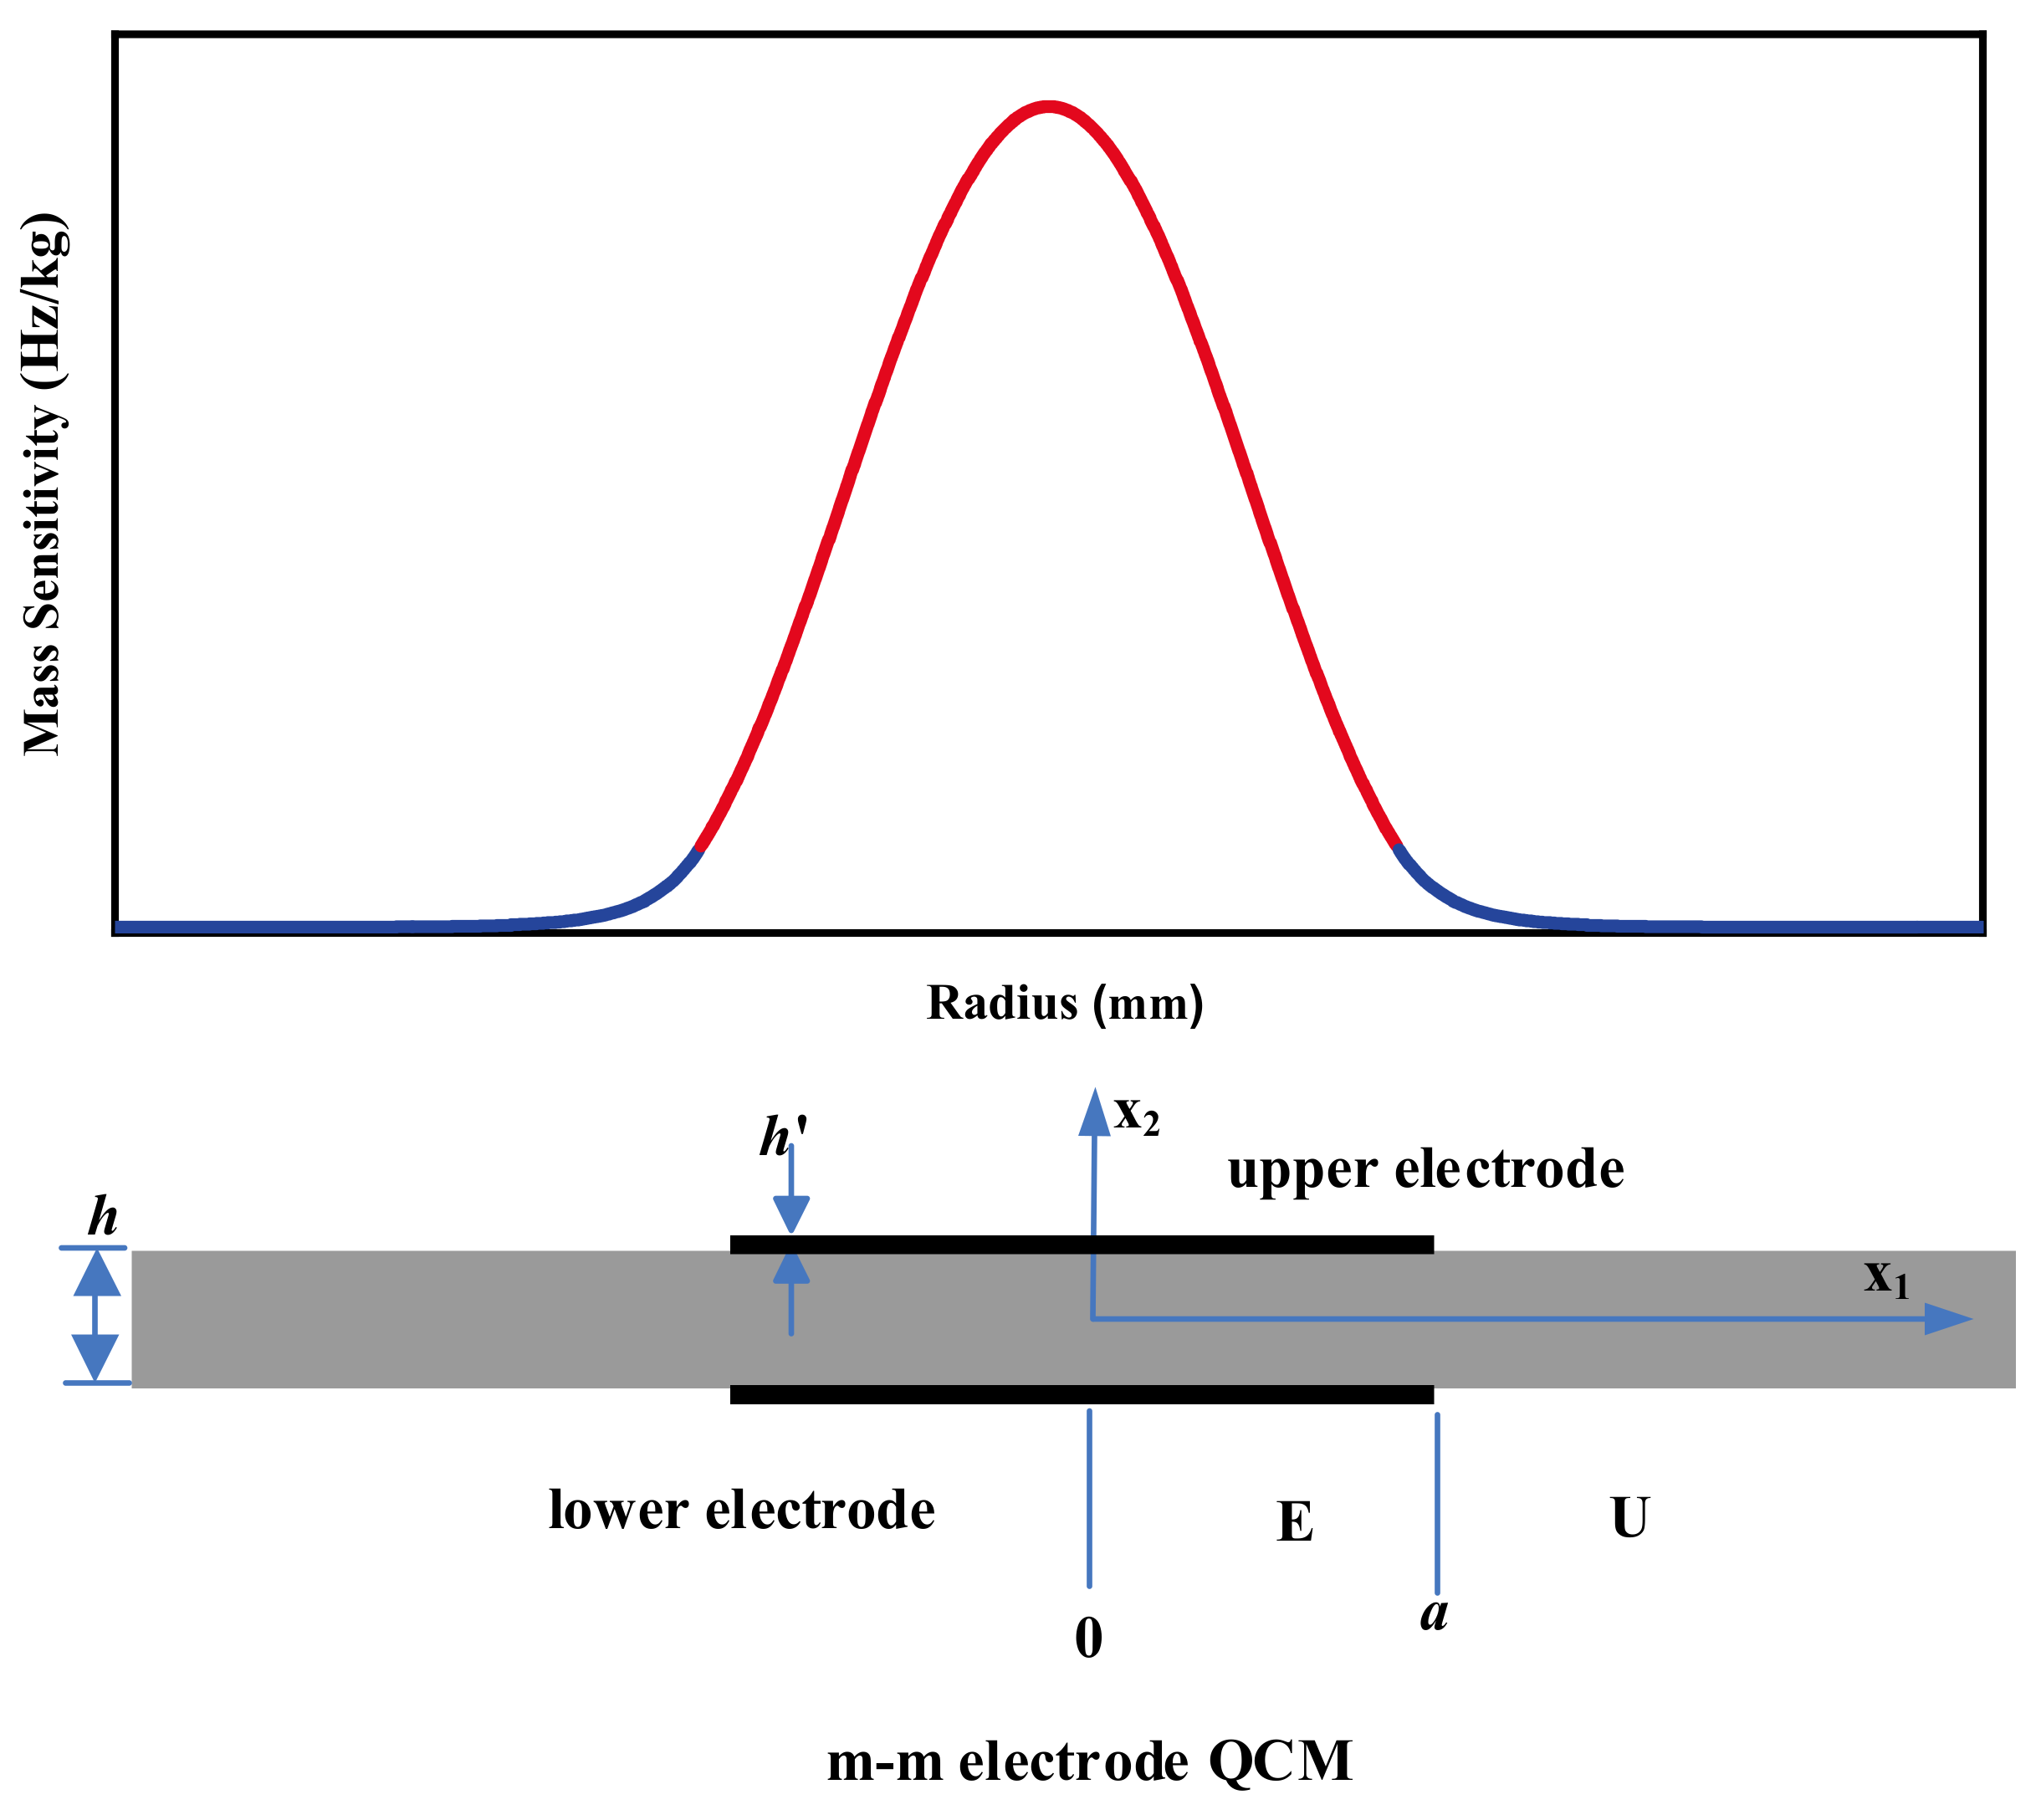
\includegraphics[width=0.8\textwidth]{assets/figures/MassSensitvity.png}
    \caption{Sensibilité de détection de la masse avec un capteur QCM \cite{Huang2022}.}
    \label{fig:mass_sensitivity}
\end{figure}

\subsection{Équation de Sauerbrey}

Développée par G. Sauerbrey en 1959 \cite{sauerbrey1959}, l’équation de Sauerbrey relie la variation de fréquence d’un cristal de quartz à la masse adsorbée sur sa surface.  
Cette équation suppose que la masse adsorbée est une extension rigide du cristal sous-jacent.

\begin{equation}
    \Delta f = -\frac{2f_0^2}{\sqrt{\mu_q \rho_q}} \cdot \frac{\Delta m}{A}
\end{equation}

\begin{itemize}[label=\textbullet]
    \item $\Delta f$ : variation de fréquence,
    \item $f_0$ : fréquence fondamentale du cristal,
    \item $\mu_q$ : module de cisaillement du quartz,
    \item $\rho_q$ : densité du quartz,
    \item $\Delta m$ : masse adsorbée,
    \item $A$ : surface du cristal.
\end{itemize}

Cependant, si la variation de fréquence dépasse 5~\% de la fréquence fondamentale, l’équation de Sauerbrey n’est plus valable.  
Il faut alors utiliser la formule de la méthode Z-match \cite{qcm100manual} :

\begin{equation}
    \Delta m = \left( \frac{N_q \cdot \rho_q}{\pi \cdot Z \cdot f_L} \right) 
    \cdot \tan^{-1} \left\{ Z \cdot \tan \left[ \pi \cdot \left( \frac{f_U - f_L}{f_U} \right) \right] \right\}
\end{equation}

Une autre relation permet de relier la fréquence et les propriétés du liquide :

\[
\Delta f = -f_u \cdot \frac{3}{2} \left( \frac{\rho_L \, \eta_L}{\pi \, \rho_q \, \mu_q} \right)^{1/2}
\]

\begin{itemize}[label=\textbullet]
    \item $f_u$ : fréquence d'oscillation du cristal non chargé,
    \item $\rho_q$ : densité du quartz : $2{,}648\, \text{g}\cdot\text{cm}^{-3}$,
    \item $\mu_q$ : module de cisaillement du quartz : $2{,}947 \times 10^{11}\, \text{g}\cdot\text{cm}^{-1}\cdot\text{s}^{-2}$,
    \item $\rho_L$ : densité du liquide en contact avec l’électrode,
    \item $\eta_L$ : viscosité du liquide en contact avec l’électrode.
\end{itemize}

\subsection{Théorie}

Dans l’article de M V. Voinova et al. \cite{M_V_Voinova_1999}, les auteurs présentent un modèle décrivant la réponse acoustique de films polymères viscoélastiques déposés sur des surfaces solides dans un environnement fluide.  
Ce modèle, basé sur l’équation des ondes, permet de calculer le décalage de la fréquence de résonance du quartz ainsi que le facteur de dissipation en fonction des propriétés viscoélastiques des couches adsorbées.

L’équation de la fréquence de résonance du quartz est :

\begin{equation}
    \delta f = \frac{1}{2\pi} \sqrt{\frac{1}{\rho_0 \cdot h_0} \cdot \frac{\omega \cdot \rho \cdot \eta}{2}}
    \label{eq:frequence_resonance}
\end{equation}

où :
\begin{itemize}[label=\textbullet]
    \item $\delta f$ : fréquence de résonance du quartz,
    \item $\rho_0$ : densité du quartz,
    \item $h_0$ : épaisseur du film adsorbé,
    \item $\omega$ : pulsation angulaire,
    \item $\rho$ : densité du liquide dans lequel le quartz est immergé,
    \item $\eta$ : viscosité du liquide.
\end{itemize}